%% ROB-GY 6003, Assignment 03: Inverse Kinematics -- report.
%% Course rules (assignments page): IEEE two-column conference format, 3 to 6 pages, US Letter.
%%   - Number all equations.
%%   - Every figure has a caption and is referenced in the text.
%%   - Label the axes of all plots.
%%   - Give units with all numbers.
%%   - No adjectives or adverbs unless backed up immediately by a quantifiable metric.
%%   - Assume the reader knows robotics but is not familiar with our class.
%% The report documents the last two goals of the assignment:
%%   (3) embed FK, IK and EE control in the robot control stack;
%%   (4) demonstrate a feedback control experiment on the robot that leverages ROS, IK and FK.
%%
%% Files: ieeeconf.cls (RAS template linked from the course page) and figures/ next to this file.
%% Data sources:
%%   fk_error.csv           ros_ws/fk_error.csv (simulator, leader-arm driving, 1980 samples)
%%   key and home poses     ros_ws/src/arm_control/arm_control/keyboard_mappings.json
%%   typing errors          press_accuracy.py tables from the lab session (real robot and simulator)
%%   teleop tracking        teleop_monitor.py output from the lab session (20 s, 600 samples)
%%   IK node test           simulator run in the lab session (/ik_target -> /true_fingertip)
%%   Fig. sim               rendered offline with LeKiwiSim and arm_control.kinematics.forward_kinematics

\documentclass[letterpaper, 10 pt, conference]{ieeeconf}

\IEEEoverridecommandlockouts
\overrideIEEEmargins

\usepackage{amsmath}
\usepackage{amssymb}
\usepackage{graphicx}
\usepackage{booktabs}
\usepackage{array}
\usepackage{xcolor}
\usepackage{url}
\usepackage{balance}
\usepackage{tikz}
\usetikzlibrary{arrows.meta}

\newcommand{\todo}[1]{\textcolor{red}{[TODO: #1]}}

\title{\LARGE \bf
Forward and Inverse Kinematics with Joint-Space Feedback\\
for Keyboard Typing on a LeKiwi Mobile Manipulator
}

\author{Ernest Saakian$^{1}$ Enkel Cerri$^{1}$ Edmond Wong$^{1}$% <- this % stops a space
\thanks{The authors are with the Tandon School of Engineering, New York University, Brooklyn, NY, USA.
        ROB-GY 6003, Team~12.
        {\tt\small es6379, ec5874, ew1697} @nyu.edu}%
}

\begin{document}

\maketitle
\thispagestyle{empty}
\pagestyle{empty}

%%%%%%%%%%%%%%%%%%%%%%%%%%%%%%%%%%%%%%%%%%%%%%%%%%%%%%%%%%%%%%%%%%%%%%%%%%%%%%%%
\begin{abstract}
Given the joint positions of a robot, how do we know the end effector position?
Given a target end effector position, how do we know which joint positions are needed to achieve it?
Forward kinematics (FK) and inverse kinematics (IK) methods can answer these exact questions.
FK is computed with a chain of frame transformations. IK is an optimization problem where we try to
minimize the difference between our predicted end effector position using FK and the target position by
adjusting the joint positions.
We set up our system as multiple ROS~2 nodes to allow our controller to drive both a simulated and a real robot.
Our FK and IK were initially validated using the simulator, and eventually we typed ``pool'' on a physical keyboard
with and without feedback.
With the arm still, the FK fingertip position matched the simulator's ground truth to within 0.011~mm on average.
On the real robot, the elbow settled 2.1--2.4$^\circ$ from its command under gravity at every key press, and
the mean key-press error was 11.6~mm with 0 of 4 keys correct. An integral correction on the joint angles
reduced it to 2.7~mm with 3 of 3 keys correct, and the robot then typed ``pool'' with 4 of 4 keys correct.
\end{abstract}

%%%%%%%%%%%%%%%%%%%%%%%%%%%%%%%%%%%%%%%%%%%%%%%%%%%%%%%%%%%%%%%%%%%%%%%%%%%%%%%%
\section{INTRODUCTION}
\label{sec:intro}

% At least one paragraph: motivation for IK and FK within the context of robot control.
When driving a robot, we have to specify the robot state in joint space where we list out the position of every single
motor on the robot \cite{c1}. The joint space does not map clearly to the end effector position, which makes it both difficult
to visualize where the robot end effector would end up and which motor positions would yield the desired end
effector position.


% One paragraph giving an overview of each section of the paper.
Section~\ref{sec:method} describes the kinematic model, the forward and inverse kinematics, and the
typing controller with joint-space feedback. Section~\ref{sec:design} details how the controller was
validated in simulation and on the robot, and how the physical measurements were taken.
Section~\ref{sec:results} presents the results, and Section~\ref{sec:conclusion} summarizes the
performance of the system.

%%%%%%%%%%%%%%%%%%%%%%%%%%%%%%%%%%%%%%%%%%%%%%%%%%%%%%%%%%%%%%%%%%%%%%%%%%%%%%%%
\section{METHOD}
\label{sec:method}

\subsection{System Overview}
\label{sec:overview}
The robot is a LeKiwi mobile manipulator~\cite{c7} (Fig.~\ref{fig:robot}): a three-wheel omnidirectional
base that carries an SO-101 arm~\cite{c4} with five revolute joints (shoulder pan, shoulder lift, elbow flex,
wrist flex and wrist roll) and a gripper. The six arm joints and the three wheels are driven by nine Feetech
STS3215 position-controlled servos on one 12~V serial bus, which a Beelink mini PC on the base reads and
commands through LeRobot~\cite{c4}. A second SO-101 arm is the leader arm for teleoperation.

All software runs as ROS~2~\cite{c2} (Jazzy) nodes on the mini PC (Fig.~\ref{fig:block},
Table~\ref{tab:nodes}). Joint angles are exchanged in degrees, followed by the gripper opening in percent.
robot\_node applies each message on
\texttt{/arm\_commands} to the servos and publishes the measured angles on \texttt{/arm\_state} at 30~Hz.
sim\_node runs the same arm in MuJoCo~\cite{c3} at 50~Hz with the same two topics, so every node in
Table~\ref{tab:nodes} runs unchanged on the simulator or on the robot. forward\_kinematics publishes the
fingertip position on \texttt{/fk\_pose} for every \texttt{/arm\_state} message. inverse\_kinematics sends
the fingertip to a position received on \texttt{/ik\_target} in a single command. keyboard\_typer receives a
letter or a word on \texttt{/key} and computes, interpolates and corrects the joint commands that press the
keys at 20~Hz.

\begin{figure}[t]
  \centering
  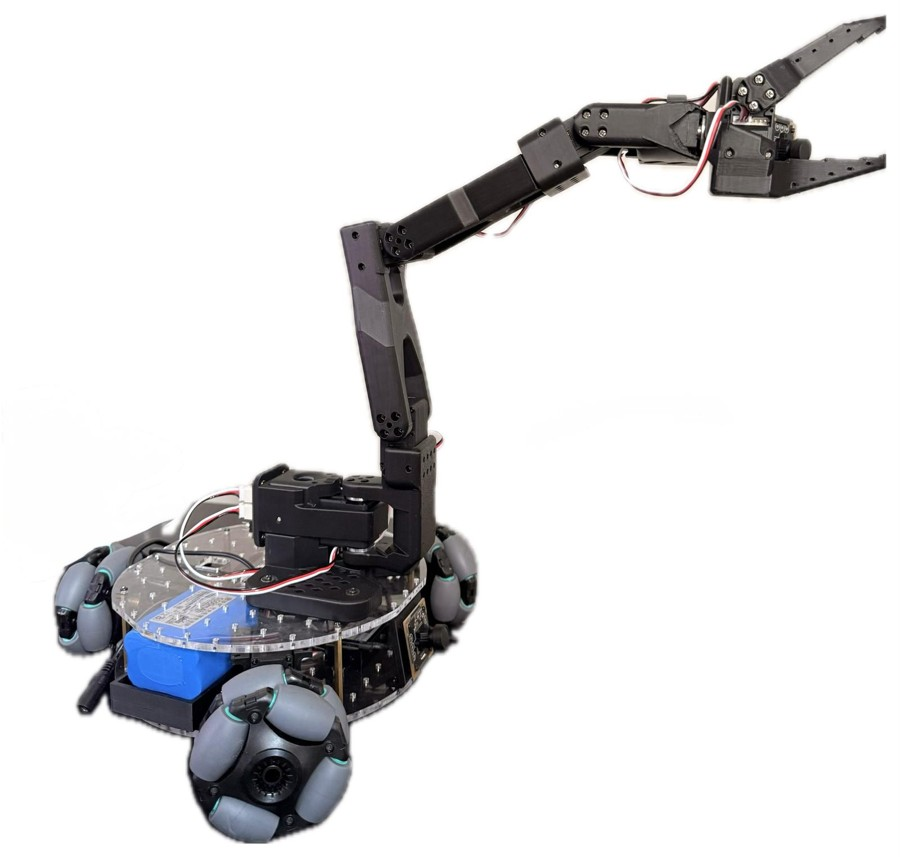
\includegraphics[width=0.38\columnwidth]{figures/robot.jpg}
  \caption{LeKiwi mobile manipulator: three-wheel omnidirectional base and SO-101 arm with five revolute
  joints and a gripper.}
  \label{fig:robot}
\end{figure}

\begin{figure}[t]
  \centering
  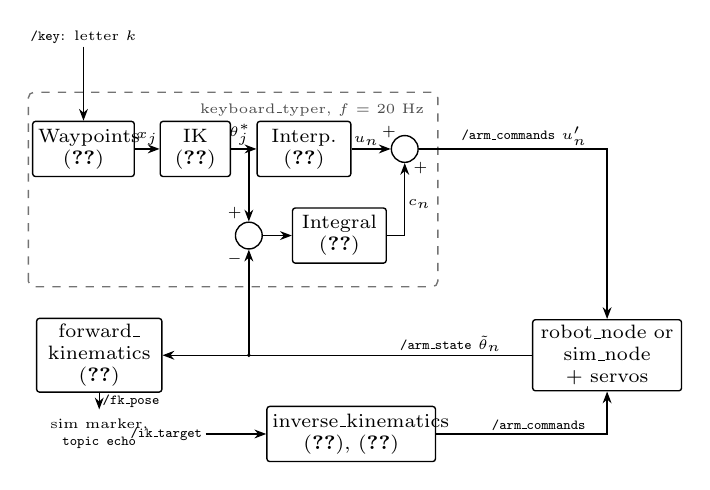
\begin{tikzpicture}[font=\scriptsize, >={Stealth[length=1.5mm]}, line width=0.5pt,
      blk/.style={draw, rounded corners=1pt, align=center, inner sep=2pt, minimum height=7mm, fill=white},
      sumn/.style={draw, circle, inner sep=0pt, minimum size=3.4mm},
      sig/.style={font=\tiny, inner sep=1pt}]
    % keyboard_typer boundary
    \draw[dashed, rounded corners=2pt, black!55] (0,-1.75) rectangle (5.2,0.72);
    \node[anchor=north east, font=\tiny, black!70] at (5.15,0.7) {keyboard\_typer, $f$ = 20~Hz};
    % blocks
    \node[blk, text width=1.15cm] (wp)    at (0.70,0)     {Waypoints\\(\ref{eq:waypoints})};
    \node[blk, text width=0.75cm] (ik)    at (2.12,0)     {IK\\(\ref{eq:ik})};
    \node[blk, text width=1.05cm] (int)   at (3.50,0)     {Interp.\\(\ref{eq:interpolation})};
    \node[sumn]                   (add)   at (4.78,0)     {};
    \node[sumn]                   (err)   at (2.80,-1.10) {};
    \node[blk, text width=1.05cm] (integ) at (3.95,-1.10) {Integral\\(\ref{eq:integral})};
    \node[blk, text width=1.75cm] (plant) at (7.35,-2.62) {robot\_node or\\sim\_node + servos};
    \node[blk, text width=1.45cm] (fk)    at (0.90,-2.62) {forward\_\\kinematics (\ref{eq:fk_position})};
    \node[blk, text width=2.0cm] (ikn)   at (4.10,-3.62) {inverse\_kinematics\\(\ref{eq:ik}), (\ref{eq:ik_accept})};
    \node[align=center, font=\tiny] (sink) at (0.90,-3.62) {sim marker,\\\texttt{topic echo}};
    % signals
    \draw[->] (0.70,1.30) node[above, sig]{\texttt{/key}: letter $k$} -- (wp.north);
    \draw[->] (wp) -- node[above, sig]{$x_j$} (ik);
    \draw[->] (ik) -- node[above, sig, pos=0.35]{$\theta_j^{*}$} (int);
    \draw[->] (int) -- node[above, sig, pos=0.38]{$u_n$} (add);
    \fill (2.80,0) circle (0.7pt);
    \draw[->] (2.80,0) -- (err.north);
    \draw[->] (err) -- (integ);
    \draw[->] (integ.east) -| node[pos=0.72, right, sig]{$c_n$} (add.south);
    \draw[->] (add.east) -| node[pos=0.28, above, sig]{\texttt{/arm\_commands} $u_n'$} (plant.north);
    \draw[->] (plant.west) -- node[pos=0.22, above, sig]{\texttt{/arm\_state} $\tilde{\theta}_n$} (fk.east);
    \fill (2.80,-2.62) circle (0.7pt);
    \draw[->] (2.80,-2.62) -- (err.south);
    \draw[->] (fk.south) -- node[right, sig]{\texttt{/fk\_pose}} (sink.north);
    \draw[->] (2.25,-3.62) node[left, sig]{\texttt{/ik\_target}} -- (ikn.west);
    \draw[->] (ikn.east) -| node[pos=0.3, above, sig]{\texttt{/arm\_commands}} (plant.south);
    % summing-junction signs
    \node[sig] at (2.62,-0.82) {$+$};
    \node[sig] at (2.62,-1.40) {$-$};
    \node[sig] at (4.58,0.22) {$+$};
    \node[sig] at (4.98,-0.24) {$+$};
  \end{tikzpicture}
  \caption{Control block diagram and ROS~2 graph. Inside keyboard\_typer (dashed box), a letter $k$ on
  \texttt{/key} becomes four fingertip waypoints $x_j$ (\ref{eq:waypoints}); each is solved by IK
  (\ref{eq:ik}), interpolated in joint space (\ref{eq:interpolation}) and corrected by the integral term
  $c_n$ (\ref{eq:integral})--(\ref{eq:corrected_command}), which acts only while a waypoint is held.
  robot\_node (or sim\_node) returns the measured angles $\tilde{\theta}_n$ on \texttt{/arm\_state}, which
  close the loop and feed forward\_kinematics. inverse\_kinematics sends a single command per
  \texttt{/ik\_target}.}
  \label{fig:block}
\end{figure}

\begin{table}[t]
\caption{ROS~2 nodes and topics}
\label{tab:nodes}
\begin{center}
\footnotesize
\setlength{\tabcolsep}{3pt}
\begin{tabular}{>{\raggedright\arraybackslash}p{2.3cm}>{\raggedright\arraybackslash}p{2.4cm}>{\raggedright\arraybackslash}p{2.7cm}}
\toprule
Node & Subscribes & Publishes \\
\midrule
robot\_node & /arm\_commands & /arm\_state \\
sim\_node & /arm\_commands, /fk\_pose & /arm\_state, /true\_fingertip, /key\_pressed \\
leader\_node & -- & /arm\_commands \\
forward\_kinematics & /arm\_state & /fk\_pose \\
inverse\_kinematics & /ik\_target, /arm\_state & /arm\_commands \\
keyboard\_typer & /key, /arm\_state & /arm\_commands \\
\bottomrule
\end{tabular}
\end{center}
\end{table}

\subsection{Kinematic Model}
\label{sec:model}
All positions are expressed in the robot's base frame $\{b\}$, with its origin at the centre of the bottom
base plate, $x$ forward (towards the arm), $y$ to the robot's left and $z$ up. The joint angles
$\theta_1,\dots,\theta_5$ belong to shoulder pan, shoulder lift, elbow flex, wrist flex and wrist roll.
The zero pose is $\theta = 0$, the middle of every joint's range. The end effector is the tip of the
gripper's fixed finger; the gripper joint moves only the other jaw and is not part of the chain. At the zero
pose the fingertip is at $p_h = (412.6, 4.8, 310.4)$~mm and the finger points along
$d_h = (0.966, 0, 0.259)$, 15.0$^\circ$ above the $x$ axis. Each joint $i$ is described by a point $q_i$ on
its axis and the unit axis direction $\hat{\omega}_i$ at the zero pose (Table~\ref{tab:joints}). A positive
$\theta_i$ turns the links after joint $i$ counter-clockwise about $\hat{\omega}_i$, so $\theta_1 > 0$
turns the arm to the robot's right. The joint limits are
$\theta_l = (-115, -100, -90, -100, -100)^\circ$ and $\theta_u = (115, 90, 95, 100, 160)^\circ$.
These parameters were read from the course's MuJoCo model, which uses the geometry of the SO-100 arm,
while the physical arm is an SO-101.

\begin{table}[t]
\caption{Joint axes at the zero pose, in the base frame}
\label{tab:joints}
\begin{center}
\begin{tabular}{lcc}
\toprule
Joint $i$ & Point $q_i$ (mm) & Axis $\hat{\omega}_i$ \\
\midrule
1 shoulder pan   & (67.2, 0.0, 84.5)   & (0, 0, $-1$) \\
2 shoulder lift  & (97.8, $-18.3$, 136.7) & (0, 1, 0) \\
3 elbow flex     & (115.8, $-16.8$, 251.2) & (0, 1, 0) \\
4 wrist flex     & (248.8, $-15.3$, 280.0) & (0, 1, 0) \\
5 wrist roll     & (307.8, 4.8, 295.8)  & ($-0.966$, 0, $-0.259$) \\
\bottomrule
\end{tabular}
\end{center}
\end{table}

\subsection{Forward Kinematics}
\label{sec:fk}
Let $\theta \in \mathbb{R}^5$ be the joint angles. For joint $i$, $[\hat{\omega}_i]$ is the
skew-symmetric matrix with $[\hat{\omega}_i]\,v = \hat{\omega}_i \times v$, and $R_i \in SO(3)$ is the
rotation by $\theta_i$ about $\hat{\omega}_i$, given by Rodrigues' formula (\ref{eq:rodrigues}). The
transform that rotates the links after joint $i$ about the axis through $q_i$ is the $4\times4$ matrix in
(\ref{eq:fk_position}). The product of these transforms from the base ($i = 1$) to the wrist ($i = 5$)
is the product-of-exponentials formula~\cite{c1}, and applied to $p_h$ it gives the fingertip position
$p(\theta)$. The finger direction $d(\theta)$ follows from the rotations alone (\ref{eq:fk_direction}).
\begin{equation}
R_i = I_3 + \sin\theta_i\,[\hat{\omega}_i] + (1-\cos\theta_i)\,[\hat{\omega}_i]^2
\label{eq:rodrigues}
\end{equation}
\begin{equation}
\begin{bmatrix} p(\theta) \\ 1 \end{bmatrix} =
\prod_{i=1}^{5} \begin{bmatrix} R_i & (I_3 - R_i)\,q_i \\ 0 & 1 \end{bmatrix}
\begin{bmatrix} p_h \\ 1 \end{bmatrix}
\label{eq:fk_position}
\end{equation}
\begin{equation}
d(\theta) = R_1 R_2 R_3 R_4 R_5\, d_h
\label{eq:fk_direction}
\end{equation}
Equation (\ref{eq:fk_position}) is the chain of homogeneous transforms of our Assignment~02 code, written with
every joint axis expressed in $\{b\}$ at the zero pose: $R_i$ rotates about an arbitrary unit axis instead of
a local $x$, $y$ or $z$ axis, and the points $q_i$ replace the link offsets. The implementation applies the
five rotations to $p_h$ and $d_h$ from $i = 5$ down to $i = 1$, which evaluates the same product from right
to left. Over 1000 random joint vectors within the limits, it differed from an explicit product of
$4\times4$ matrices by at most 1.8~$\mu$m, from the 5-digit rounding of $\hat{\omega}_5$. The forward\_kinematics node evaluates
(\ref{eq:fk_position}) for every \texttt{/arm\_state} message and publishes $p(\tilde{\theta})$ as a
\texttt{PoseStamped} in frame \texttt{base} on \texttt{/fk\_pose}. sim\_node subscribes to
\texttt{/fk\_pose} and draws a magenta sphere of 8~mm radius at that point (Fig.~\ref{fig:sim}).

\subsection{Inverse Kinematics}
\label{sec:ik}
Given a desired fingertip position $p_d$ and finger direction $d_d$, IK solves the bounded optimization
(\ref{eq:ik}). Here $\theta_l$ and $\theta_u$ are the joint limits, $w = 0.05$~m weights the dimensionless
direction error against the position error in metres, and $d_d = -e_3$ (finger straight down) for every
target in this work, with $e_3 = (0, 0, 1)$. The solver is SciPy's~\cite{c5} bounded quasi-Newton method
L-BFGS-B~\cite{c6} with finite-difference gradients and at most 500 iterations, started from $\theta_0$:
the current measured angles or the previous waypoint's solution. A solution $\theta^{*}$ is accepted only if
(\ref{eq:ik_accept}) holds with $\epsilon = 5$~mm; otherwise the target is reported as unreachable and no
command is sent.
\begin{equation}
\theta^{*} = \arg\min_{\theta_l \le \theta \le \theta_u}
\lVert p_d - p(\theta) \rVert + w\,\lVert d_d - d(\theta) \rVert
\label{eq:ik}
\end{equation}
\begin{equation}
\lVert p_d - p(\theta^{*}) \rVert \le \epsilon
\label{eq:ik_accept}
\end{equation}
Two properties of the model shape this problem. First, $d_h$ is parallel to $\hat{\omega}_5$, so
$\theta_5$ does not change $d(\theta)$. Second, $\hat{\omega}_2 = \hat{\omega}_3 = \hat{\omega}_4$ and
$R_1$ leaves $e_3$ unchanged, so the tilt $\varphi$ of the finger from $-e_3$ depends on three joints only:
\begin{equation}
\varphi = \left| \theta_2 + \theta_3 + \theta_4 - 105^\circ \right|
\label{eq:tilt}
\end{equation}
The target therefore fixes four quantities (three position coordinates and $\varphi = 0$) with five joints.
$\theta_5$ still moves the fingertip, because $p_h$ lies 13.0~mm from the wrist-roll axis, so the solver
optimizes all five angles, and $\theta_0$ selects one of the remaining solutions.

\subsection{Keyboard Typing Controller}
\label{sec:typing}
Let $x_k \in \mathbb{R}^3$ be the recorded position of the top of key $k$ and $x_H$ the recorded home
position, both in $\{b\}$ (Section~\ref{sec:mapping}). keyboard\_typer accepts one letter or a word on
\texttt{/key}; spaces are ignored, a message that contains an unmapped letter is rejected before the arm
moves, and a message that arrives while a word is being typed is ignored. For each letter $k$ it builds the
four fingertip waypoints (\ref{eq:waypoints}): above the key at hover height $h$, below the key top at press
depth $\delta$, above the key again, and home. Each waypoint $j = 1,\dots,4$ is solved with (\ref{eq:ik})
for $p_d = x_j$ and $d_d = -e_3$, started from the previous solution, which keeps consecutive joint
targets $\theta_j^{*}$ close together. $\theta_0^{*}$ is the measured angle vector when the letter starts.
If any waypoint fails (\ref{eq:ik_accept}), the letter and the rest of the word are not typed.
\begin{equation}
x_1 = x_k + h\,e_3, \quad x_2 = x_k - \delta\,e_3, \quad x_3 = x_1, \quad x_4 = x_H
\label{eq:waypoints}
\end{equation}
The node runs at $f = 20$~Hz. At step $n$ of move $j$, counted from the step at which move $j$ starts, the
command $u_n \in \mathbb{R}^5$ interpolates linearly in joint space from $\theta_{j-1}^{*}$ to
$\theta_j^{*}$ over $N = T_m f$ steps (\ref{eq:interpolation}), where $T_m$ is the duration of one move.
The waypoint is then held for $T_s f$ further steps before move $j+1$ starts. The gripper command is 0~\%
(closed) throughout. Because every letter ends at $x_H$, the single message ``pool'' produces the sequence
p--home--o--home--o--home--l. One letter takes $4(T_m + T_s) = 15.2$~s on the robot, plus 0.37~s per IK
solve on the mini PC.
\begin{equation}
u_n = \theta_{j-1}^{*} + \left(\theta_j^{*} - \theta_{j-1}^{*}\right) \min\!\left(1, \frac{n}{N}\right),
\quad N = T_m f
\label{eq:interpolation}
\end{equation}

\subsection{Joint-Space Feedback Correction}
\label{sec:feedback}
Each STS3215 servo closes a proportional position loop internally; LeRobot sets its proportional coefficient
to 16, half of the default 32, to reduce oscillation. Under a constant load torque, such as gravity on the
links or the spring of a pressed key, a proportional loop settles where the torque from the position error
balances the load, so the joint settles at an offset from its command in the direction of the load. Without
correction, the elbow settled 2.1--2.4$^\circ$ from its command in the direction of gravity at every key press
(Section~\ref{sec:results}).

keyboard\_typer therefore adds an integral correction $c_n \in \mathbb{R}^5$ to the interpolated command.
Let $\tilde{\theta}_n$ be the latest measured joint angles from \texttt{/arm\_state}, $K$ the integral gain
per step, and $\operatorname{sat}_{c_m}$ the element-wise clipping to $[-c_m, c_m]$. While waypoint $j$ is
held ($N \le n \le N + T_s f$), the joint error is accumulated (\ref{eq:integral}), and the published
command is (\ref{eq:corrected_command}):
\begin{equation}
c_n =
\begin{cases}
\operatorname{sat}_{c_m}( c_{n-1} + K ( \theta_j^{*} - \tilde{\theta}_n ) ), & N \le n \le N + T_s f \\
c_{n-1}, & n < N
\end{cases}
\label{eq:integral}
\end{equation}
\begin{equation}
u_n' = u_n + c_n
\label{eq:corrected_command}
\end{equation}
$c$ is zero when the node starts and is not reset between waypoints or letters, so each move starts with the
correction learned at the previous waypoint. In steady state $c_n = c_{n-1}$ requires
$\tilde{\theta} = \theta_j^{*}$, so a constant load leaves no steady-state joint error as long as
$\lvert c \rvert < c_m$. If the servo reached each new command within one step, the error would decay as
$(1-K)^n$, to 7~\% of its initial value after the $T_s f = 16$ steps of a hold. The limit $c_m = 4^\circ$ per
joint bounds the extra command, which limits how far the finger is pushed into the keyboard when a target
cannot be reached and stops the integral from winding up. Table~\ref{tab:params} lists the parameters.

\begin{table}[t]
\caption{Controller parameters}
\label{tab:params}
\begin{center}
\footnotesize
\begin{tabular}{l>{\raggedright\arraybackslash}p{3.4cm}ll}
\toprule
Symbol & Meaning & Robot & Sim. \\
\midrule
$w$        & direction weight in (\ref{eq:ik})  & 0.05~m & 0.05~m \\
$\epsilon$ & IK acceptance threshold            & 5~mm   & 5~mm \\
$h$        & hover height above key             & 40~mm  & 40~mm \\
$\delta$   & press depth below key top          & 5.5~mm$^{\dagger}$ & 8~mm \\
$T_m$      & duration of one move               & 3.0~s  & 1.5~s \\
$f$        & command rate of keyboard\_typer    & 20~Hz  & 20~Hz \\
$T_s$      & hold time at each waypoint         & 0.8~s  & 0.8~s \\
$K$        & integral gain per step             & 0.15   & 0.15 \\
$c_m$      & correction limit per joint         & 4$^\circ$ & 4$^\circ$ \\
--         & robot\_node / sim\_node rate       & 30~Hz  & 50~Hz \\
--         & robot\_node step limit             & 15$^\circ$ & -- \\
\bottomrule
\multicolumn{4}{l}{\scriptsize $^{\dagger}$2.5~mm and 4~mm in the two measured runs (Section~\ref{sec:typing_exp}).}
\end{tabular}
\end{center}
\end{table}

%%%%%%%%%%%%%%%%%%%%%%%%%%%%%%%%%%%%%%%%%%%%%%%%%%%%%%%%%%%%%%%%%%%%%%%%%%%%%%%%
\section{EXPERIMENT DESIGN}
\label{sec:design}

\subsection{Hardware and Software Setup}
Experimentation was done both on hardware and simulation. Our hardware setup was an onboard computer, an SO-101
follower arm~\cite{c4} on a LeKiwi base~\cite{c7}, as well as the SO-101 leader arm. While only the follower arm
and the keyboard were necessary, it was observed that recording positions of the keyboard keys was more accurately
done with teleoperation with the leader arm instead of just moving the follower arm into place physically and then
just recording the position (Section~\ref{sec:mapping}). The SO-101 is the robot placed to the right of a full-size
keyboard, with the arm facing it (Fig.~\ref{fig:setup}). Which key registered was read from the characters typed
on the computer the keyboard is connected to. For simulation we used MuJoCo~\cite{c3}. Our MuJoCo setup involves an
environment with a virtual keyboard with 3 keys, a, s and d, whose caps are 24~mm wide and 70~mm apart (a
physical keyboard has a key pitch of 19.05~mm); they travel 6~mm and register at 3~mm (Fig.~\ref{fig:sim}a).

\begin{figure}[t]
  \centering
  \begin{tikzpicture}
    \node[anchor=south west, inner sep=0] (img) at (0,0)
      {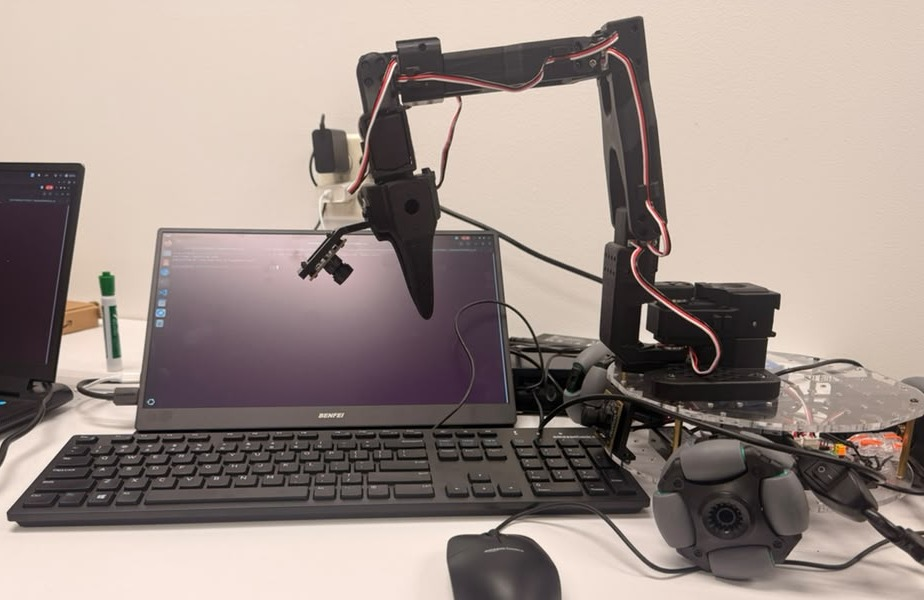
\includegraphics[width=\columnwidth]{figures/setup.jpg}};
    \begin{scope}[x={(img.south east)}, y={(img.north west)}, >={Stealth[length=1.6mm]}]
      % P, O and L keys
      \foreach \px/\py in {0.332/0.243, 0.361/0.243, 0.335/0.223}
        {\draw[white, line width=1.4pt] (\px,\py) circle (2.2pt);
         \draw[orange, line width=0.7pt] (\px,\py) circle (2.2pt);}
      \draw[white, line width=1.4pt] (0.345,0.205) -- (0.30,0.07);
      \draw[orange, line width=0.7pt] (0.345,0.205) -- (0.30,0.07);
      \node[fill=white, inner sep=1.5pt, font=\scriptsize, anchor=north] at (0.30,0.07) {P, O, L keys};
      % fingertip at the home position
      \draw[white, line width=1.4pt] (0.454,0.47) circle (2.6pt);
      \draw[orange, line width=0.7pt] (0.454,0.47) circle (2.6pt);
      \node[fill=white, inner sep=1.5pt, font=\scriptsize, anchor=west] at (0.49,0.47) {$x_H$};
      % base frame (schematic)
      \foreach \ex/\ey/\lab/\pos in {0.67/0.30/x/left, 0.83/0.47/z/above, 0.77/0.19/y/below}
        {\draw[->, white, line width=1.8pt] (0.83,0.30) -- (\ex,\ey);
         \draw[->, orange, line width=0.8pt] (0.83,0.30) -- (\ex,\ey)
           node[\pos, fill=white, inner sep=1pt, font=\scriptsize] {$\lab$};}
    \end{scope}
  \end{tikzpicture}
  \caption{Experimental setup. The LeKiwi stands to the right of the keyboard with the arm facing it and the
  fingertip at the home position $x_H$, 98.7~mm above the mean height of the recorded P, O and L key tops.
  The base-frame axes are drawn schematically at the robot's base; $y$ points towards the camera.}
  \label{fig:setup}
\end{figure}

\subsection{Forward Kinematics Validation in Simulation}
The simulator was started with the typing launch file (sim\_node with the keyboard scene, forward\_kinematics,
inverse\_kinematics and keyboard\_typer), and the simulated arm was driven with the leader arm through
leader\_node for 39.6~s. The marker drawn at \texttt{/fk\_pose} was checked visually against the fingertip
(Fig.~\ref{fig:sim}). For a number, a logger subscribed to \texttt{/fk\_pose} and to
\texttt{/true\_fingertip}, the position of the simulator's fingertip site in $\{b\}$, and paired each
\texttt{/fk\_pose} message with the \texttt{/true\_fingertip} message closest in time, within 10~ms
(sim\_node publishes every 20~ms). For each pair it recorded the FK error (\ref{eq:fk_error}), where
$p_{gt}$ is the simulator's fingertip and $\tilde{\theta}$ the joint angles of the same simulation step.
Pairing by timestamp matters: in a scripted joint sweep, pairing the latest message of each topic instead
produced a maximum error of 54~mm, against 2.7~mm with timestamp pairing.
\begin{equation}
e_{FK} = \lVert p(\tilde{\theta}) - p_{gt} \rVert
\label{eq:fk_error}
\end{equation}

\begin{figure}[t]
  \centering
  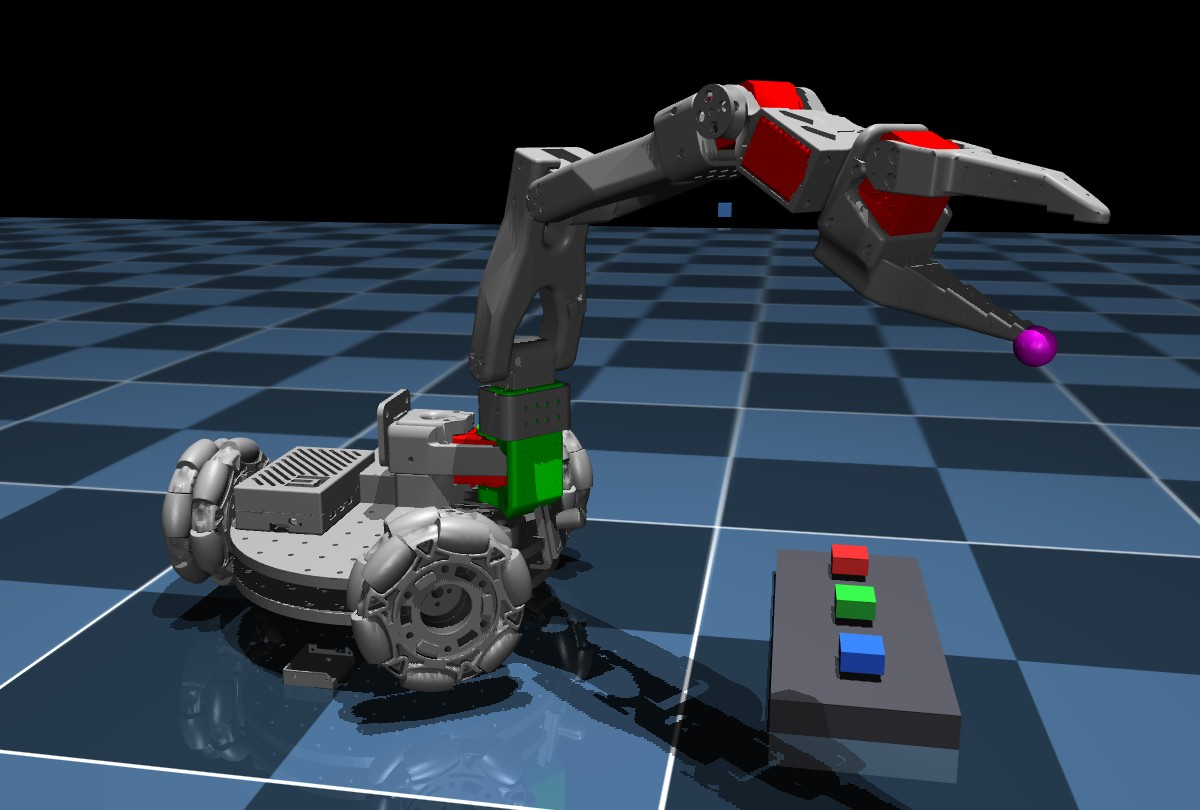
\includegraphics[width=0.49\columnwidth]{figures/sim_fk_wide.jpg}\hfill
  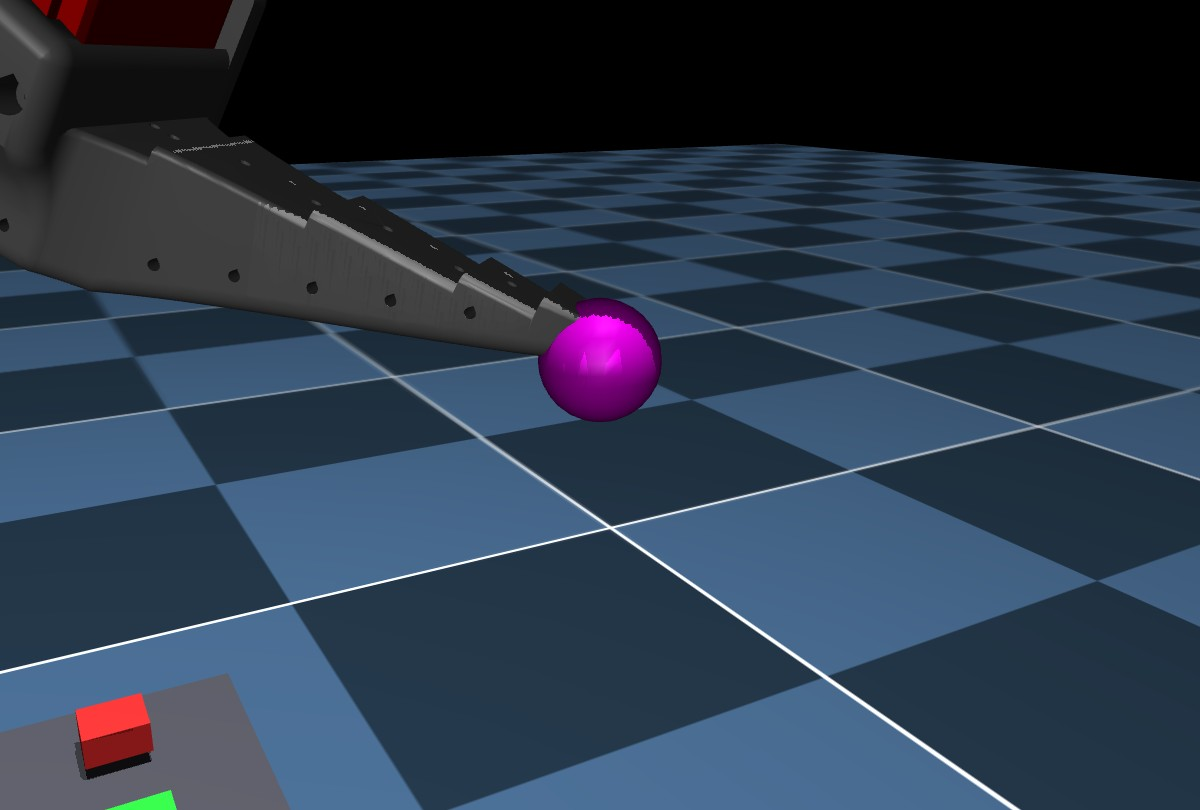
\includegraphics[width=0.49\columnwidth]{figures/sim_fk_close.jpg}\\[1pt]
  \makebox[0.49\columnwidth]{\footnotesize (a)}\hfill\makebox[0.49\columnwidth]{\footnotesize (b)}
  \caption{FK marker in the simulator for $\theta = (40, 20, -30, 50, 0)^\circ$. The magenta sphere (8~mm
  radius) is drawn at $p(\tilde{\theta})$ from (\ref{eq:fk_position}), the point sim\_node draws for
  \texttt{/fk\_pose}; rendered offline with the simulator's own rendering and marker code. (a) Arm and
  the simulated keys a, s and d. (b) Close-up of the fixed finger; $p(\tilde{\theta})$ is 0.006~mm from
  the simulator's fingertip.}
  \label{fig:sim}
\end{figure}

\subsection{Keyboard Mapping}
\label{sec:mapping}
To map the keyboard keys, the robot was initially moved by hand to the position of each key; however, there was
an issue with this. When moving the robot by hand, the robot's position also included the robot's flex as the hand
dragged the robot towards the correct position; this movement was not related to the servos' positions, so it was
not picked up. A better way to map the keyboard was to teleoperate the robot instead; this ensures that the robot
has reached a position because its servos carried it there. With the motors on and robot\_node at 30~Hz with a
15$^\circ$ step limit, the follower was driven with the leader arm until the fingertip rested on top of each key
without pressing it, and the positions were recorded using \texttt{ros2 topic echo} on the topics
\texttt{/fk\_pose} and \texttt{/arm\_state} (Table~\ref{tab:keys}). In addition we recorded a home position above
the keyboard. The robot and keyboard were not moved between the mapping and the typing runs.

\subsection{End-Effector Control}
For the purposes of testing inverse kinematics, individual positions were published on \texttt{/ik\_target}. The
inverse\_kinematics node solves (\ref{eq:ik}) from the current \texttt{/arm\_state} with $d_d = -e_3$ and sends the
solution to \texttt{/arm\_commands} in one message; if the error exceeds $\epsilon = 5$~mm
(\ref{eq:ik_accept}), the target is treated as unreachable and refused. This test was run in the simulator only:
three targets were published 6~s apart, $(280, 50, 50)$~mm, the home position $(266, 19, 90)$~mm and
$(900, 0, 300)$~mm, which is outside the arm's reach, and the fingertip position was read from
\texttt{/true\_fingertip} after each move. For keyboard typing, the inverse kinematics code was used as a library
and the robot was controlled by the keyboard\_typer node (Section~\ref{sec:typing}).

\subsection{Typing Experiments and Accuracy Measurement}
\label{sec:typing_exp}
Typing accuracy was measured with a logger node that subscribes to \texttt{/key}, \texttt{/arm\_commands} and
\texttt{/arm\_state} without publishing. It evaluates (\ref{eq:fk_position}) for every \texttt{/arm\_state}
message, detects a press as an interval in which the fingertip is more than 1~mm below the lowest key top,
takes the sample $n'$ with the lowest fingertip in each interval, and reports the horizontal press error
(\ref{eq:press_error}), where $[I_2\;\,0]$ selects the $x$ and $y$ components, and the depth below the press
target $x_k - \delta e_3$. $e_p$ is computed from the measured joint angles through the model; it includes the
servo errors but not the error of the model itself, for which no external measurement was available. Whether
the intended key registered was read from the characters typed on the computer (robot) and from
\texttt{/key\_pressed} (simulator).
\begin{equation}
e_{p} = \left\lVert \begin{bmatrix} I_2 & 0 \end{bmatrix}
\left( p(\tilde{\theta}_{n'}) - x_k + \delta\,e_3 \right) \right\rVert
\label{eq:press_error}
\end{equation}

Four conditions were measured, each with letters sent one at a time:
\begin{itemize}
\item Simulator, $K = 0$ and $K = 0.15$: keys a, s, d, with all other parameters as in Table~\ref{tab:params}.
\item Robot, $K = 0$: keys p, o, o, l with the controller as it was before the correction was added. This
version had no hold phase ($T_s = 0$) and used $\delta = 2.5$~mm.
\item Robot, $K = 0.15$: $T_s = 0.8$~s and $\delta = 4$~mm. The run contained six presses; the logger
matches letters to presses in order, and only the first three, p, o and l, could be matched to the letter
that was sent, so only those three are reported.
\end{itemize}
Both robot runs used $T_m = 3.0$~s and robot\_node at 30~Hz with a 15$^\circ$ step limit. In the $K = 0$ run
the logger used the FK of the commanded press angles as the target, which equals $x_k - \delta e_3$ because the
IK error was 0.0~mm. The final run, recorded
on video, sent the single message ``pool'' with $K = 0.15$, $\delta = 5.5$~mm and $T_m = 3.0$~s, without the
logger.

%%%%%%%%%%%%%%%%%%%%%%%%%%%%%%%%%%%%%%%%%%%%%%%%%%%%%%%%%%%%%%%%%%%%%%%%%%%%%%%%
\section{EXPERIMENTAL RESULTS}
\label{sec:results}

\subsection{Forward Kinematics Accuracy}
Fig.~\ref{fig:fk_error} shows $e_{FK}$ over the 39.6~s run (1980 samples), and Table~\ref{tab:fk} splits it
by fingertip speed, with ``still'' meaning below 5~mm/s. With the arm still, $e_{FK}$ was 0.011~mm on
average and at most 0.021~mm, the size of the rounding in the model parameters. While the arm moved, the mean
rose to 0.598~mm and the maximum to 1.90~mm. This error comes from the simulator, not from the FK: MuJoCo
computes site positions at the start of each 2~ms physics step, before it integrates the joint angles, so
\texttt{/true\_fingertip} belongs to the joint angles of the previous physics step. The fingertip speed
times 2~ms follows $e_{FK}$ with a correlation coefficient of 0.97 (Fig.~\ref{fig:fk_error}). In an offline
sweep, recomputing the site positions for the current joint angles reduced the error from 1.16~mm to
0.006~mm on average (0.008~mm maximum).

\begin{figure}[t]
  \centering
  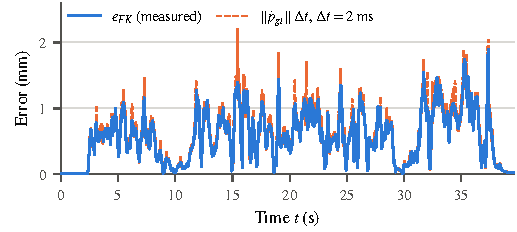
\includegraphics[width=\columnwidth]{figures/fk_error.pdf}
  \caption{FK error $e_{FK}$ (\ref{eq:fk_error}) against the simulator's fingertip while the arm was driven
  with the leader arm, and the fingertip speed $\lVert\dot{p}_{gt}\rVert$ multiplied by the 2~ms physics
  step. Both are in mm; the FK error while moving matches the one-step reporting lag of the simulator.}
  \label{fig:fk_error}
\end{figure}

\begin{table}[t]
\caption{FK error against simulator ground truth}
\label{tab:fk}
\begin{center}
\footnotesize
\setlength{\tabcolsep}{4pt}
\begin{tabular}{lcccc}
\toprule
Condition & Samples & Mean (mm) & 95th pct. (mm) & Max (mm) \\
\midrule
Arm still  & 116  & 0.011 & 0.011 & 0.021 \\
Arm moving & 1863 & 0.598 & 1.196 & 1.896 \\
All        & 1980 & 0.563 & 1.187 & 1.896 \\
\bottomrule
\end{tabular}
\end{center}
\end{table}

\subsection{Teleoperation and Joint Tracking}
\label{sec:teleop}
With robot\_node at its default 10~Hz, \texttt{/arm\_state} arrived at 10~Hz while leader\_node published
\texttt{/arm\_commands} at 30~Hz, so the arm applied one command in three and moved in 100~ms steps.
LeRobot also clips every goal to within the step limit of the joint's present position, which at 5$^\circ$
per step capped each joint at 50$^\circ$/s. With \texttt{rate\_hz} set to 30~Hz both topics ran at 30.2~Hz,
but in a 20~s recording the joints that lift weight stalled: shoulder lift was commanded from $-103.9^\circ$
to $79.5^\circ$ and moved from $-103.4^\circ$ to $-87.1^\circ$, the elbow reached 46.4$^\circ$ of a
99.2$^\circ$ command and wrist flex $-13.6^\circ$ of $-0.7^\circ$, while shoulder pan, which turns about a
vertical axis, stayed within 3.4$^\circ$ of its command. Because the clipping is relative to the present
position, a lagging joint's servo never sees more than 5$^\circ$ of error, which at a proportional
coefficient of 16 did not produce the torque to lift the arm. The step limit was raised to 15$^\circ$ for all
later runs. The tracking test was not repeated, but in the typing run without correction shoulder lift was
within 2.7$^\circ$ of its command at every press.

\subsection{Key Positions}
Table~\ref{tab:keys} lists the recorded positions. Evaluating (\ref{eq:fk_position}) on the recorded
\texttt{/arm\_state} reproduced each recorded \texttt{/fk\_pose} within 0.3~mm. By (\ref{eq:tilt}) the
finger was tilted 15.9$^\circ$, 17.2$^\circ$ and 19.2$^\circ$ from vertical on P, O and L, and 8.8$^\circ$ at
home. The home position is 98.7~mm above the mean key-top height, inside the 50--100~mm band the assignment
asks for, but 89.4~mm from the centroid of the three keys towards the robot instead of above it; it was kept
because IK reaches it from every key with 0.0~mm error. The recorded points are 20.8~mm (P--O), 22.1~mm (O--L) and 32.7~mm (P--L) apart horizontally,
against 19.1, 19.6 and 23.8~mm between key centres at a 19.05~mm key pitch; the 1.7--8.9~mm differences combine
where on each cap the fingertip rested with the error of the SO-100 model on the SO-101 arm.

\begin{table}[t]
\caption{Recorded key and home positions in the base frame}
\label{tab:keys}
\begin{center}
\begin{tabular}{lccc}
\toprule
Pose & $x$ (mm) & $y$ (mm) & $z$ (mm) \\
\midrule
P    & 347.0 & 10.1 & $-10.0$ \\
O    & 364.1 & 21.9 & $-7.4$ \\
L    & 354.7 & 42.0 & $-9.7$ \\
Home & 266.0 & 19.3 & 89.7 \\
\bottomrule
\end{tabular}
\end{center}
\end{table}

\subsection{Inverse Kinematics and End-Effector Control}
Table~\ref{tab:ik} shows the \texttt{/ik\_target} test in the simulator. The node refused $(900, 0, 300)$~mm
and the arm stayed at the previous position. The two reachable targets were missed by 7.5~mm and 6.0~mm,
5.1--6.0~mm of it in $z$, because the simulated joints also stop short of their commands under gravity; for
example, at the pose of Fig.~\ref{fig:sim} shoulder lift settled at 21.5$^\circ$ for a 20.0$^\circ$ command. The inverse\_kinematics node has no
correction, so it shows the same steady-state error as keyboard\_typer with $K = 0$ in simulation
(4.6--5.5~mm, Table~\ref{tab:typing}).

For typing, all twelve waypoints of P, O and L, solved in sequence from the recorded home angles, met
(\ref{eq:ik_accept}) with a position error below 0.05~mm. The finger tilt $\varphi$ was 16--21$^\circ$ at the
key waypoints and 0$^\circ$ at home, and consecutive waypoints differed by 11--41$^\circ$ in the joint that moved
most. The tilt comes from (\ref{eq:ik}): its norms are not squared, so the cost is not differentiable at
zero position error, where L-BFGS-B stops without reducing $\varphi$. Squaring both terms (in mm) reduced the
tilt to at most 3$^\circ$ in an offline check, but turned the wrist roll by 113--154$^\circ$ on the first move,
so the unsquared cost was kept.

\begin{table}[t]
\caption{End-effector control with the inverse\_kinematics node (simulator)}
\label{tab:ik}
\begin{center}
\begin{tabular}{lcc}
\toprule
Target (mm) & Reached (mm) & Error (mm) \\
\midrule
(280, 50, 50)  & (275.6, 49.1, 44.0) & 7.5 \\
(266, 19, 90)  & (262.9, 18.8, 84.9) & 6.0 \\
(900, 0, 300)  & refused             & -- \\
\bottomrule
\end{tabular}
\end{center}
\end{table}

\subsection{Typing Accuracy Without and With Feedback}
Fig.~\ref{fig:typing} and Table~\ref{tab:typing} compare the press error without and with the correction.
On the robot without correction, all four presses landed 10.3--11.9~mm from the target towards the robot,
which on this keyboard is the key to the right: P pressed P and [ together, both O presses pressed P, and L
pressed the semicolon. 0 of 4 keys were correct. In all four presses the elbow settled 2.1--2.4$^\circ$ from its
command in the direction that lowers the fingertip. Linearizing (\ref{eq:fk_position}) at the recorded key poses, $+1^\circ$ of elbow moves
the fingertip 3.6--3.8~mm towards the robot and 2.7--2.9~mm down, so the elbow error alone accounts for
7.5--9.0~mm of the displacement, and wrist-flex errors of up to 1.1$^\circ$ add up to 3.1~mm. The fingertip also
went 5.2--7.2~mm deeper than the press target.

With $K = 0.15$, the error fell to 2.1--3.1~mm (mean 2.7~mm, 77~\% lower), the fingertip stopped
0.6--0.7~mm above the press target, and 3 of 3 keys were correct. In the simulator the mean fell from 5.0~mm
to 0.7~mm (86~\% lower), and all three keys registered in both conditions. In two of the robot presses the
measured shoulder-lift angle exceeded its corrected command by 5.5--5.7$^\circ$. Because $\lvert c \rvert \le 4^\circ$,
at least 1.5--1.7$^\circ$ of shoulder-lift error from $\theta_j^{*}$ remained, so a larger $c_m$ could reduce
the remaining error.
In the final run, the message ``pool'' produced p, o, o, l on the computer with 4 of 4 keys correct.

The robot conditions also differ in the hold phase and in $\delta$ (Section~\ref{sec:typing_exp}); in the
simulator, $K = 0$ included the 0.8~s hold and still missed by 4.6--5.5~mm.

\begin{figure}[t]
  \centering
  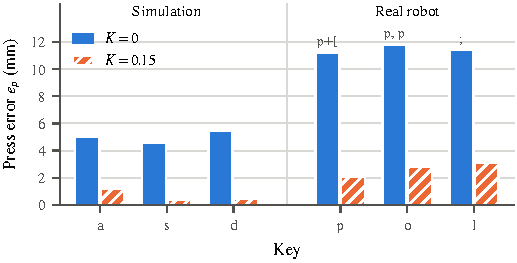
\includegraphics[width=\columnwidth]{figures/typing_error.pdf}
  \caption{Press error $e_p$ (\ref{eq:press_error}) per key without ($K = 0$) and with ($K = 0.15$) the
  joint-space correction, in the simulator (keys a, s, d) and on the robot (keys p, o, l). The robot's
  $K = 0$ bar for o is the mean of two presses (11.9 and 11.7~mm). Labels above the robot's $K = 0$ bars give
  the key that went down instead.}
  \label{fig:typing}
\end{figure}

\begin{table}[t]
\caption{Key-press error $e_p$}
\label{tab:typing}
\begin{center}
\footnotesize
\begin{tabular}{lccc}
\toprule
Condition & Mean (mm) & Max (mm) & Keys correct \\
\midrule
Sim., $K = 0$       & 5.0  & 5.5  & 3 / 3 \\
Sim., $K = 0.15$    & 0.7  & 1.2  & 3 / 3 \\
Robot, $K = 0$      & 11.6 & 11.9 & 0 / 4 \\
Robot, $K = 0.15$   & 2.7  & 3.1  & 3 / 3 \\
Robot, ``pool'' & -- & -- & 4 / 4 \\
\bottomrule
\end{tabular}
\end{center}
\end{table}

% Balances the two columns of the last page; must be issued in the LEFT column of that page.
\balance
\subsection{Problems and Assumptions}
Unlike the robot in the simulation, the real SO-101 is made of 3D-printed plastic, and the gears in the servos
have some backlash. This means that there is always going to be some degree of free movement that goes on without
being controlled or detected by the servos. With an open-loop control where we just tell the robot to go to certain
coordinates, we cannot guarantee that we reach the same point on every attempt. This error is also magnified by the
keyboard and robot not being fixed to the desk, so they can move between experiments, which resulted in multiple
attempts to achieve success.

The command rate and the step limit of robot\_node had to be raised from 10 to 30~Hz and from 5 to
15$^\circ$ (Section~\ref{sec:teleop}). Before the key
mapping, the six arm servos were found to hold the leader arm's calibration offsets. robot\_node checks them
only with the motors on, so in read-only mode it had reported $-124^\circ$ (shoulder lift) and $-137^\circ$
(elbow) for the folded arm, against $-110.0^\circ$ and $96.9^\circ$ after the robot's calibration was written
back. All real-robot data in this report were taken after that.

The kinematic model describes the SO-100 arm, so $p(\theta)$ and $e_p$ on the SO-101 are not ground truth
(Section~\ref{sec:typing_exp}), and the robot comparison is one run per condition, with 4 and 3 presses.

%%%%%%%%%%%%%%%%%%%%%%%%%%%%%%%%%%%%%%%%%%%%%%%%%%%%%%%%%%%%%%%%%%%%%%%%%%%%%%%%
\section{CONCLUSION}
\label{sec:conclusion}
FK, IK, the end-effector controller and the typing controller run as ROS~2 nodes that drive the simulated
and the real LeKiwi without changes. In the simulator the FK matched the true fingertip to 0.011~mm with the
arm still, and IK solved every typing waypoint to below 0.05~mm. On the robot, open-loop joint commands were
not enough to type: the elbow settled 2.1--2.4$^\circ$ from its command under gravity, the fingertip missed by
11.6~mm on average, and 0 of 4 keys were correct. Integral feedback on the measured joint angles cut the miss
to 2.7~mm and made 3 of 3 measured presses and 4 of 4 letters of ``pool'' correct.

The parts that limited performance were the servos' steady-state error under load, the 5$^\circ$ default step
limit, which held shoulder lift to 16.3$^\circ$ of a 183.4$^\circ$ command, the 4$^\circ$ correction limit,
which left 1.5--1.7$^\circ$ of shoulder-lift error, the 16--21$^\circ$ finger tilt of the IK solutions, and
the time per letter, 15.2~s. Next steps are to measure the fingertip on the robot with a camera or ruler,
calibrate the model to the SO-101, repeat the with/without comparison with identical $\delta$ and $T_s$ and
more presses, raise $c_m$, and use a squared IK cost with a penalty on wrist-roll motion.

%%%%%%%%%%%%%%%%%%%%%%%%%%%%%%%%%%%%%%%%%%%%%%%%%%%%%%%%%%%%%%%%%%%%%%%%%%%%%%%%
\begin{thebibliography}{99}

\bibitem{c1} K.~M. Lynch and F.~C. Park, \emph{Modern Robotics: Mechanics, Planning, and Control}.
Cambridge, U.K.: Cambridge Univ. Press, 2017.

\bibitem{c2} S.~Macenski, T.~Foote, B.~Gerkey, C.~Lalancette, and W.~Woodall, ``Robot Operating
System 2: Design, architecture, and uses in the wild,'' \emph{Science Robotics}, vol.~7, no.~66, 2022.

\bibitem{c3} E.~Todorov, T.~Erez, and Y.~Tassa, ``MuJoCo: A physics engine for model-based control,''
in \emph{Proc. IEEE/RSJ Int. Conf. Intelligent Robots and Systems (IROS)}, 2012, pp.~5026--5033.

\bibitem{c4} R.~Cadene \emph{et al.}, ``LeRobot: State-of-the-art machine learning for real-world
robotics in PyTorch,'' 2024. [Online]. Available: \url{https://github.com/huggingface/lerobot}

\bibitem{c5} P.~Virtanen \emph{et al.}, ``SciPy 1.0: Fundamental algorithms for scientific computing
in Python,'' \emph{Nature Methods}, vol.~17, pp.~261--272, 2020.

\bibitem{c6} R.~H. Byrd, P.~Lu, J.~Nocedal, and C.~Zhu, ``A limited memory algorithm for bound
constrained optimization,'' \emph{SIAM J. Scientific Computing}, vol.~16, no.~5, pp.~1190--1208, 1995.

\bibitem{c7} SIGRobotics-UIUC, ``LeKiwi: Low-cost mobile manipulator,'' 2025. [Online]. Available:
\url{https://github.com/SIGRobotics-UIUC/LeKiwi}

\end{thebibliography}

\end{document}
